\documentclass{ximera}

 

\usepackage{epsfig}

\graphicspath{
  {./}
  {figures/}
}

\usepackage{morewrites}
\makeatletter
\newcommand\subfile[1]{%
\renewcommand{\input}[1]{}%
\begingroup\skip@preamble\otherinput{#1}\endgroup\par\vspace{\topsep}
\let\input\otherinput}
\makeatother

\newcommand{\includeexercises}{\directlua{dofile("/home/jim/linearAlgebra/laode/exercises.lua")}}

%\newcounter{ccounter}
%\setcounter{ccounter}{1}
%\newcommand{\Chapter}[1]{\setcounter{chapter}{\arabic{ccounter}}\chapter{#1}\addtocounter{ccounter}{1}}

%\newcommand{\section}[1]{\section{#1}\setcounter{thm}{0}\setcounter{equation}{0}}

%\renewcommand{\theequation}{\arabic{chapter}.\arabic{section}.\arabic{equation}}
%\renewcommand{\thefigure}{\arabic{chapter}.\arabic{figure}}
%\renewcommand{\thetable}{\arabic{chapter}.\arabic{table}}

%\newcommand{\Sec}[2]{\section{#1}\markright{\arabic{ccounter}.\arabic{section}.#2}\setcounter{equation}{0}\setcounter{thm}{0}\setcounter{figure}{0}}

\newcommand{\Sec}[2]{\section{#1}}

\setcounter{secnumdepth}{2}
%\setcounter{secnumdepth}{1} 

%\newcounter{THM}
%\renewcommand{\theTHM}{\arabic{chapter}.\arabic{section}}

\newcommand{\trademark}{{R\!\!\!\!\!\bigcirc}}
%\newtheorem{exercise}{}

\newcommand{\dfield}{{\sf dfield9}}
\newcommand{\pplane}{{\sf pplane9}}

\newcommand{\EXER}{\section*{Exercises}}%\vspace*{0.2in}\hrule\small\setcounter{exercise}{0}}
\newcommand{\CEXER}{}%\vspace{0.08in}\begin{center}Computer Exercises\end{center}}
\newcommand{\TEXER}{} %\vspace{0.08in}\begin{center}Hand Exercises\end{center}}
\newcommand{\AEXER}{} %\vspace{0.08in}\begin{center}Hand Exercises\end{center}}

% BADBAD: \newcommand{\Bbb}{\bf}

\newcommand{\R}{\mbox{$\Bbb{R}$}}
\newcommand{\C}{\mbox{$\Bbb{C}$}}
\newcommand{\Z}{\mbox{$\Bbb{Z}$}}
\newcommand{\N}{\mbox{$\Bbb{N}$}}
\newcommand{\D}{\mbox{{\bf D}}}
\usepackage{amssymb}
%\newcommand{\qed}{\hfill\mbox{\raggedright$\square$} \vspace{1ex}}
%\newcommand{\proof}{\noindent {\bf Proof:} \hspace{0.1in}}

\newcommand{\setmin}{\;\mbox{--}\;}
\newcommand{\Matlab}{{M\small{AT\-LAB}} }
\newcommand{\Matlabp}{{M\small{AT\-LAB}}}
\newcommand{\computer}{\Matlab Instructions}
\newcommand{\half}{\mbox{$\frac{1}{2}$}}
\newcommand{\compose}{\raisebox{.15ex}{\mbox{{\scriptsize$\circ$}}}}
\newcommand{\AND}{\quad\mbox{and}\quad}
\newcommand{\vect}[2]{\left(\begin{array}{c} #1_1 \\ \vdots \\
 #1_{#2}\end{array}\right)}
\newcommand{\mattwo}[4]{\left(\begin{array}{rr} #1 & #2\\ #3
&#4\end{array}\right)}
\newcommand{\mattwoc}[4]{\left(\begin{array}{cc} #1 & #2\\ #3
&#4\end{array}\right)}
\newcommand{\vectwo}[2]{\left(\begin{array}{r} #1 \\ #2\end{array}\right)}
\newcommand{\vectwoc}[2]{\left(\begin{array}{c} #1 \\ #2\end{array}\right)}

\newcommand{\ignore}[1]{}


\newcommand{\inv}{^{-1}}
\newcommand{\CC}{{\cal C}}
\newcommand{\CCone}{\CC^1}
\newcommand{\Span}{{\rm span}}
\newcommand{\rank}{{\rm rank}}
\newcommand{\trace}{{\rm tr}}
\newcommand{\RE}{{\rm Re}}
\newcommand{\IM}{{\rm Im}}
\newcommand{\nulls}{{\rm null\;space}}

\newcommand{\dps}{\displaystyle}
\newcommand{\arraystart}{\renewcommand{\arraystretch}{1.8}}
\newcommand{\arrayfinish}{\renewcommand{\arraystretch}{1.2}}
\newcommand{\Start}[1]{\vspace{0.08in}\noindent {\bf Section~\ref{#1}}}
\newcommand{\exer}[1]{\noindent {\bf \ref{#1}}}
\newcommand{\ans}{}
\newcommand{\matthree}[9]{\left(\begin{array}{rrr} #1 & #2 & #3 \\ #4 & #5 & #6
\\ #7 & #8 & #9\end{array}\right)}
\newcommand{\cvectwo}[2]{\left(\begin{array}{c} #1 \\ #2\end{array}\right)}
\newcommand{\cmatthree}[9]{\left(\begin{array}{ccc} #1 & #2 & #3 \\ #4 & #5 &
#6 \\ #7 & #8 & #9\end{array}\right)}
\newcommand{\vecthree}[3]{\left(\begin{array}{r} #1 \\ #2 \\
#3\end{array}\right)}
\newcommand{\cvecthree}[3]{\left(\begin{array}{c} #1 \\ #2 \\
#3\end{array}\right)}
\newcommand{\cmattwo}[4]{\left(\begin{array}{cc} #1 & #2\\ #3
&#4\end{array}\right)}

\newcommand{\Matrix}[1]{\ensuremath{\left(\begin{array}{rrrrrrrrrrrrrrrrrr} #1 \end{array}\right)}}

\newcommand{\Matrixc}[1]{\ensuremath{\left(\begin{array}{cccccccccccc} #1 \end{array}\right)}}



\renewcommand{\labelenumi}{\theenumi)}
\newenvironment{enumeratea}%
{\begingroup
 \renewcommand{\theenumi}{\alph{enumi}}
 \renewcommand{\labelenumi}{(\theenumi)}
 \begin{enumerate}}
 {\end{enumerate}\endgroup}



\newcounter{help}
\renewcommand{\thehelp}{\thesection.\arabic{equation}}

%\newenvironment{equation*}%
%{\renewcommand\endequation{\eqno (\theequation)* $$}%
%   \begin{equation}}%
%   {\end{equation}\renewcommand\endequation{\eqno \@eqnnum
%$$\global\@ignoretrue}}

%\input{psfig.tex}

\author{Martin Golubitsky and Michael Dellnitz}

%\newenvironment{matlabEquation}%
%{\renewcommand\endequation{\eqno (\theequation*) $$}%
%   \begin{equation}}%
%   {\end{equation}\renewcommand\endequation{\eqno \@eqnnum
% $$\global\@ignoretrue}}

\newcommand{\soln}{\textbf{Solution:} }
\newcommand{\exercap}[1]{\centerline{Figure~\ref{#1}}}
\newcommand{\exercaptwo}[1]{\centerline{Figure~\ref{#1}a\hspace{2.1in}
Figure~\ref{#1}b}}
\newcommand{\exercapthree}[1]{\centerline{Figure~\ref{#1}a\hspace{1.2in}
Figure~\ref{#1}b\hspace{1.2in}Figure~\ref{#1}c}}
\newcommand{\para}{\hspace{0.4in}}

\renewenvironment{solution}{\suppress}{\endsuppress}

\ifxake
\newenvironment{matlabEquation}{\begin{equation}}{\end{equation}}
\else
\newenvironment{matlabEquation}%
{\let\oldtheequation\theequation\renewcommand{\theequation}{\oldtheequation*}\begin{equation}}%
  {\end{equation}\let\theequation\oldtheequation}
\fi

\makeatother


\title{Matrices of Linear Maps on a Vector Space}

\begin{document}
\begin{abstract}
\end{abstract}
\maketitle

  \label{MALT}
\index{linear}  \index{coordinates}


Returning to the general finite dimensional vector space $V$, suppose that
\[
{\cal W} = \{w_1,\ldots,w_n\} \AND {\cal Z} = \{z_1,\ldots,z_n\}
\]
are bases of $V$.  Then we can write
\[
v = \alpha_1 w_1 + \cdots + \alpha_n w_n \AND
v = \beta_1 z_1 + \cdots + \beta_n z_n
\]
to obtain the coordinates
\begin{equation}  \label{e:vincoords}
[v]_{\cal W} = (\alpha_1,\ldots,\alpha_n) \AND
[v]_{\cal Z} = (\beta_1,\ldots,\beta_n)
\end{equation}
of $v$ relative to the bases ${\cal W}$ and ${\cal Z}$.  The question that
we address is: How are $[v]_{\cal W}$ and $[v]_{\cal Z}$ related?  We answer
this question by finding an $n\times n$ matrix $C_{{\cal W}{\cal Z}}$ such that
\begin{equation} \label{e:coordchange}
\vect{\alpha}{n} = C_{{\cal W}{\cal Z}} \vect{\beta}{n}.
\end{equation}
We may rewrite \Ref{e:coordchange} as
\begin{equation}  \label{e:coordchange2}
[v]_{\cal W} = C_{{\cal W}{\cal Z}}[v]_{\cal Z}.
\end{equation}

\begin{definition}
Let ${\cal W}$ and ${\cal Z}$ be bases\index{basis} for the $n$-dimensional
vector space $V$.  The $n\times n$ matrix $C_{{\cal W}{\cal Z}}$
is a {\em transition\/} matrix if $C_{{\cal W}{\cal Z}}$ satisfies
\Ref{e:coordchange2}.
\end{definition}  \index{matrix!transition}


\subsubsection*{Transition Mappings Defined}

The next theorem presents a method for finding the transition matrix
between coordinates associated to bases in an $n$-dimensional vector
space $V$.

\begin{theorem}  \label{T:coordform}
Let ${\cal W}=\{w_1,\ldots,w_n\}$ and ${\cal Z}=\{z_1,\ldots,z_n\}$
be bases for the $n$-dimensional vector space\index{vector!space} $V$.
Then
\begin{equation} \label{e:coordform}
C_{{\cal W}{\cal Z}} =
\left(\begin{array}{ccc} c_{11} & \cdots & c_{1n} \\
\vdots & \vdots & \vdots \\
c_{n1} & \cdots & c_{nn} \end{array}\right)
\end{equation}
is the transition matrix, where
\begin{equation} \label{e:wtoz}
\begin{array}{ccc}
z_1 & = & c_{11}w_1 + \cdots + c_{n1}w_n \nonumber \\
    & \vdots &  \\
z_n & = & c_{1n}w_1 + \cdots + c_{nn}w_n \nonumber
\end{array}
\end{equation}
for scalars $c_{ij}$.
\end{theorem}

\begin{proof}
We can restate \Ref{e:wtoz} as
\[
[z_j]_{\cal W} = \left(\begin{array}{c} c_{1j} \\ \vdots \\c_{nj}
\end{array} \right).
\]
Note that
\[
[z_j]_{\cal Z} = e_j,
\]
by definition.  Since the transition matrix satisfies
$[v]_{\cal W} =  C_{{\cal W}{\cal Z}}[v]_{\cal Z}$ for all vectors
$v\in V$, it must satisfy this relation for $v=z_j$.  Therefore,
\[
[z_j]_{\cal W} = C_{{\cal W}{\cal Z}}[z_j]_{\cal Z} = C_{{\cal W}{\cal Z}}e_j.
\]
It follows that $[z_j]_{\cal W}$ is the $j^{th}$ column of
$C_{{\cal W}{\cal Z}}$, which proves the theorem.  \end{proof}

\subsubsection*{A Formula for $C_{\cal WZ}$ when $V=\R^n$}

For bases in $\R^n$, there is a formula for finding transition
matrices\index{matrix!transition}.  Let ${\cal W} =\{w_1,\ldots,w_n\}$
and ${\cal Z} = \{z_1,\ldots,z_n\}$ be bases of $\R^n$ --- written as row
vectors.
Also, let $v\in\R^n$ be written as a row vector.  Then \Ref{e:coordRn}
implies that
\[
[v]_{\cal W} = P_{\cal W}\inv v^t \AND [v]_{\cal Z} = P_{\cal Z}\inv v^t,
\]
where
\[
P_{\cal W} = (w_1^t|\cdots|w_n^t) \AND  P_{\cal Z} = (z_1^t|\cdots|z_n^t).
\]
It follows that
\[
[v]_{\cal W} = P_{\cal W}\inv P_{\cal Z} [v]_{\cal Z}
\]
and that
\begin{equation} \label{e:coordformn}
C_{\cal WZ} = P_{\cal W}\inv P_{\cal Z}.
\end{equation}

As an example, consider the following bases of $\R^4$.  Let
\begin{equation*}
\begin{array}{ccccccc}
w_1 & = & [1, 4, 2, 3] & \hspace{0.2in} & z_1 & = & [3, 2, 0, 1] \\
w_2 & = & [2, 1, 1, 4] &  		    & z_2 & = & [-1, 0, 2, 3] \\
w_3 & = & [0, 1, 5, 6] & 		    & z_3 & = & [3, 1, 1, 3] \\
w_4 & = & [2, 5, -1, 0] & 		    & z_4 & = & [2, 2, 3, 5]
\end{array}
\end{equation*}
Then the matrix $C_{\cal WZ}$ is obtained by typing {\tt e9\_4\_7} to
enter the bases and
\begin{verbatim}
inv([w1' w2' w3' w4'])*[z1' z2' z3' z4']
\end{verbatim}
to compute $C_{\cal WZ}$.  The answer is:
\begin{verbatim}
ans =
   -8.0000    5.5000   -7.0000   -3.2500
   -0.5000    0.7500    0.0000    0.1250
    4.5000   -2.7500    4.0000    2.3750
    6.0000   -4.0000    5.0000    2.5000
\end{verbatim}



\subsubsection*{Coordinates Relative to Two Different Bases in $\R^2$}

Recall the basis ${\cal W}$
\[
w_1=(1,1) \AND w_2=(1,-2)
\]
of $\R^2$ that was used in a previous example.  Suppose that
${\cal Z}=\{z_1,z_2\}$ is a second basis of $\R^2$.  Write $v=(v_1,v_2)$
as a linear combination of the basis ${\cal Z}$
\[
v=\beta_1z_1 + \beta_2z_2,
\]
obtaining the coordinates $[v]_{\cal Z}=(\beta_1,\beta_2)$.

We use \Matlab to illustrate how the coordinates of a vector $v$ relative
to two bases may be viewed geometrically.  Suppose that $z_1=(1,3)$ and
$z_2=(1,-2)$.  Then enter the two bases ${\cal W}$ and ${\cal Z}$ by typing
\begin{verbatim}
w1 = [1 1];
w2 = [1 -2];
z1 = [1 3];
z2 = [-1 2];
ccoord
\end{verbatim}


The \Matlab program {\sf ccoord}\index{\computer!ccoord} opens two
graphics windows
representing the ${\cal W}$ and ${\cal Z}$ planes with the basis
vectors plotted in red.  Clicking the left mouse button on a
vector in the ${\cal W}$ plane simultaneously plots this vector
$v$ in both planes in yellow and the coordinates of $v$ in the
respective bases in cyan.  See Figure~\ref{F:2coords}.  From
this display you can visualize the coordinates of a
vector relative to two different bases.

\begin{figure}[htb]
     \centerline{%
     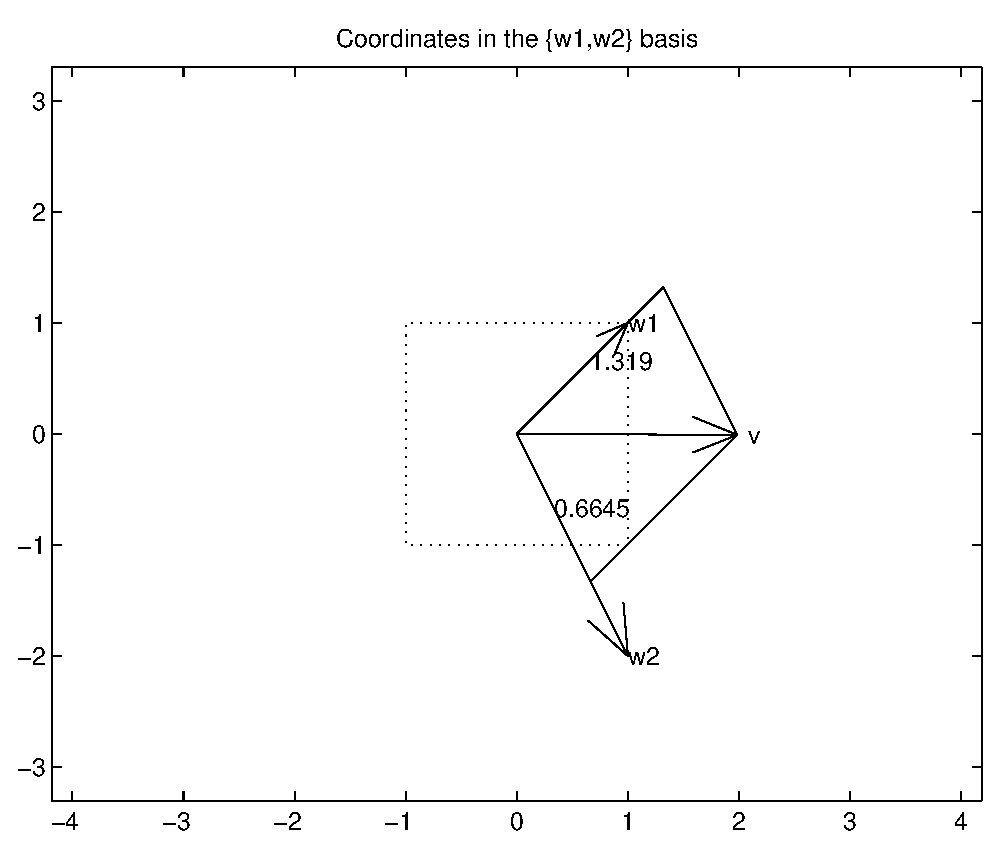
\psfig{file=../figures/ccoorda.eps,width=3.0in}
	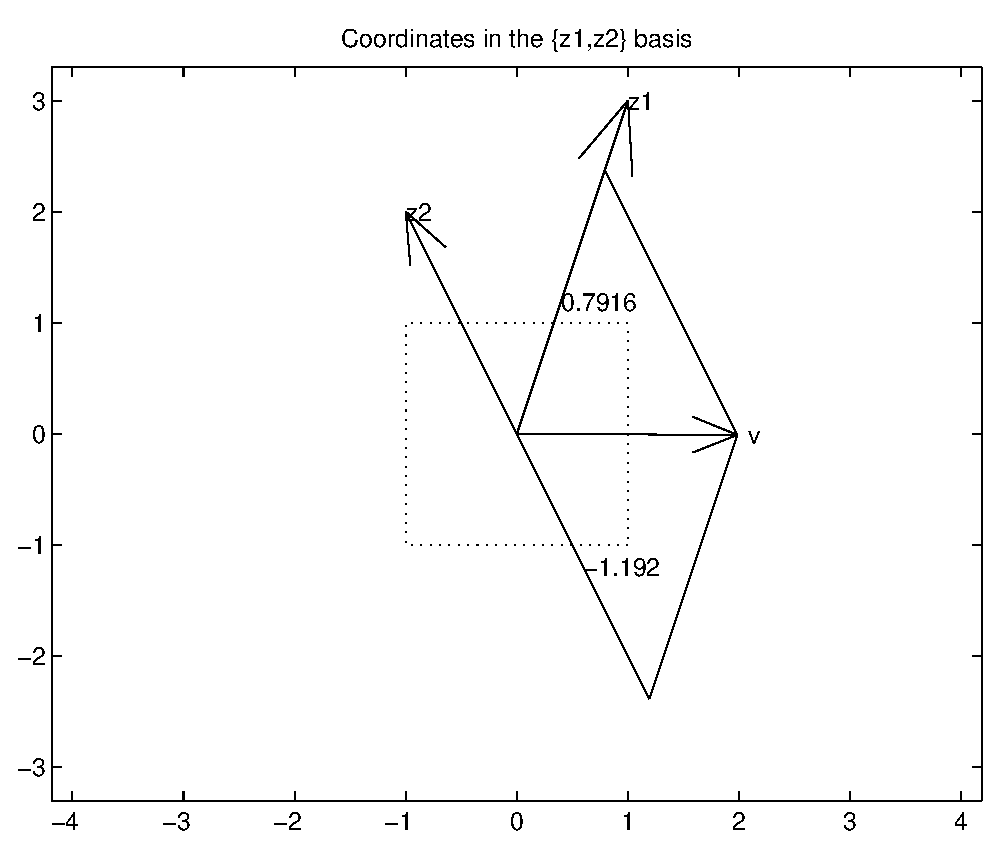
\psfig{file=../figures/ccoordb.eps,width=3.0in}}
     \caption{The coordinates of $v=(1.9839,-0.0097)$ in the bases
	$w_1=(1,1), w_2=(1,-2)$ and $z_1=(1,3),z_2=(-1,2)$.}
     \label{F:2coords}
\end{figure}

Note that the program {\sf ccoord} prints the transition matrix
$C_{\cal WZ}$ in the \Matlab control window.  We can verify the
calculations of the program {\sf ccoord} on this example by hand.
Recall that \Ref{e:coordformn} states that
\begin{eqnarray*}
C_{\cal WZ} & = & \mattwo{1}{2}{2}{3}\inv\mattwo{1}{2}{4}{1} \\
& = & \mattwo{-3}{2}{2}{-1}\mattwo{1}{2}{4}{1} \\
& = & \mattwo{5}{-4}{-2}{3}.
\end{eqnarray*}


\subsection*{Matrices of Linear Maps in Different Bases}

\begin{theorem} \label{T:matrixcoord}
Let $L:V\to V$ be a linear mapping\index{linear!mapping} and let
${\cal W}$ and ${\cal Z}$ be bases of $V$.  Then
\[
[L]_{\cal Z} \AND [L]_{\cal W}
\]
are similar \index{similar} matrices.  More precisely,
\begin{equation}  \label{e:matrixcoord}
[L]_{\cal W} = C_{{\cal Z}{\cal W}}\inv [L]_{\cal Z} C_{{\cal Z}{\cal W}}.
\end{equation}
\end{theorem}

\begin{proof}  For every $v\in\R^n$ we compute
\begin{eqnarray*}
C_{{\cal Z}{\cal W}}[L]_{\cal W}[v]_{\cal W} & = &
C_{{\cal Z}{\cal W}}[L(v)]_{\cal W} \\
& = & [L(v)]_{\cal Z}  \\
& = & [L]_{\cal Z}[v]_{\cal Z} \\
& = & [L]_{\cal Z} C_{{\cal Z}{\cal W}}[v]_{\cal W}.
\end{eqnarray*}
Since this computation holds for every $[v]_{\cal W}$, it follows that
\[
C_{{\cal Z}{\cal W}}[L]_{\cal W} = [L]_{\cal Z} C_{{\cal Z}{\cal W}}.
\]
Thus \Ref{e:matrixcoord} is valid.  \end{proof}





\EXER

\TEXER

\begin{exercise} \label{c7.1.2}
Let
\[
w_1 = (1,2) \AND w_2 = (0,1)
\]
and
\[
z_1 = (2,3) \AND z_2 = (3,4)
\]
be two bases of $\R^2$.  Find $C_{WZ}$.
\end{exercise}



\begin{exercise} \label{c7.3.2}
Let $f_1(t)=\cos t$ and $f_2(t)=\sin t$ be functions in $\CCone$.
Let $V$ be the two dimensional subspace spanned by $f_1,f_2$; so
${\cal F}=\{f_1,f_2\}$ is a basis for $V$.  Let $L:V\to V$ be the
linear mapping defined by $L(f)=\frac{df}{dt}$.  Find $[L]_{\cal F}$.
\end{exercise}

\begin{exercise} \label{c7.3.3}
Let $L:V\to W$ and $M:W\to V$ be linear mappings, and assume $\dim V > \dim W$.
Show that $M\compose L:V\to V$ is not invertible.
\end{exercise}

\CEXER

\begin{exercise} \label{c7.1.5}
Let
\[
w_1 = (0.23,0.56) \AND w_2 = (0.17,-0.71)
\]
and
\[
z_1 = (-1.4,0.3) \AND z_2 = (0.1,-0.2)
\]
be two bases of $\R^2$ and let $v=(0.6,0.1)$.  Find $[v]_{\cal
W}$, $[v]_{\cal Z}$, and $C_{\cal WZ}$.
\end{exercise}

\begin{exercise}  \label{c7.5.A}
Consider the matrix
\begin{equation*}
A = \frac{1}{3}\left(\begin{array}{ccc}
	1 & 1-\sqrt{3} & 1+\sqrt{3} \\
	1+\sqrt{3} & 1 & 1-\sqrt{3} \\
	1-\sqrt{3} & 1+\sqrt{3} & 1
	\end{array}\right)
  =  \left(\begin{array}{rrr}
    0.3333  & -0.2440  &  0.9107\\
    0.9107  &  0.3333  & -0.2440\\
   -0.2440  &  0.9107  &  0.3333
 \end{array}\right)
\end{equation*}
\begin{itemize}
\item[(a)]  Try to determine the way that the matrix $A$ moves vectors
in $\R^3$.  For example, let
\[
w_1=(1,1,1)^t \qquad w_2 = \frac{1}{\sqrt{6}}(1,-2,1)^t \qquad w_3 =
\frac{1}{\sqrt{2}}(1,0,-1)^t
\]
and compute $Aw_j$.
\item[(b)]  Let ${\cal W} = \{w_1,w_2,w_3\}$ be the basis of $\R^3$ given
in (a).  Compute $[L_A]_{\cal W}$.
\item[(c)]  Determine the way that the matrix $[L_A]_{\cal W}$ moves 
vectors in $\R^3$.  For example, consider how this matrix moves the standard 
basis vectors $e_1,e_2,e_3$.  Compare this answer with that in part (a).
\end{itemize}
\end{exercise}

\end{document}
